\usepackage{amsmath}
\usetikzlibrary{calc,positioning,arrows.meta}

\newcommand{\systolicarrowstyle}{-{Latex[length=1.45mm,width=0.95mm]}}

\newcommand{\drawpecell}[3]{%
\begin{tikzpicture}[
    font=\small,
    sig/.style={\systolicarrowstyle, line width=0.9pt, line cap=round, line join=round},
    cell/.style={draw, line width=1.0pt, minimum size=1.85cm},
    diagcell/.style={draw, double, double distance=1.2pt, line width=0.95pt, minimum size=1.85cm},
    rbox/.style={draw, line width=0.85pt, minimum width=5.5mm, minimum height=4.8mm, inner sep=0.5pt}
]
  \node[#1] (cellbox) at (0,0) {};
  \node[font=\ttfamily] at ($(cellbox.center)+(0,0.22)$) {#2};
  \node[rbox] at ($(cellbox.center)+(0,-0.38)$) {$\text{r}$};

  \draw[sig] (0,1.95) node[above] {$\text{data\_i}$} -- (cellbox.north);
  \draw[sig] (cellbox.south) -- (0,-1.95) node[below] {$\text{data\_o}$};
  \draw[sig] (-2.05,0) node[left] {$\text{#3}$} -- (cellbox.west);
  \draw[sig] (cellbox.east) -- (2.05,0) node[right] {$\text{op\_o}$};
  \draw[sig] (-2.05,0.72) node[left] {$\text{clk}$} -- (-0.925,0.72);
\end{tikzpicture}%
}

\newcommand{\drawpecellwithreduce}[3]{%
\begin{tikzpicture}[
    font=\small,
    sig/.style={\systolicarrowstyle, line width=0.9pt, line cap=round, line join=round},
    redsig/.style={\systolicarrowstyle, line width=0.9pt, line cap=round, line join=round},
    cell/.style={draw, line width=1.0pt, minimum size=1.85cm},
    rbox/.style={draw, line width=0.85pt, minimum width=5.5mm, minimum height=4.8mm, inner sep=0.5pt}
]
  \node[cell] (cellbox) at (0,0) {};
  \node[font=\ttfamily] at ($(cellbox.center)+(0,0.22)$) {#2};
  \node[rbox] at ($(cellbox.center)+(0,-0.38)$) {$\text{r}$};

  \draw[sig] (0,1.95) node[above] {$\text{data\_i}$} -- (cellbox.north);
  \draw[sig] (cellbox.south) -- (0,-1.95) node[below] {$\text{data\_o}$};
  \draw[sig] (-2.05,0) node[left] {$\text{#3}$} -- (cellbox.west);
  \draw[sig] (cellbox.east) -- (2.05,0) node[right] {$\text{op\_o}$};
  \draw[sig] (-2.05,0.72) node[left] {$\text{clk}$} -- (-0.925,0.72);

  \draw[redsig] (-2.05,1.95) node[above left] {$\text{reduce\_sig\_i}$} -- (cellbox.north west);
  \draw[redsig] (cellbox.south east) -- (2.05,-1.95) node[below right] {$\text{reduce\_sig\_o}$};
\end{tikzpicture}%
}

\newcommand{\drawdelayline}{%
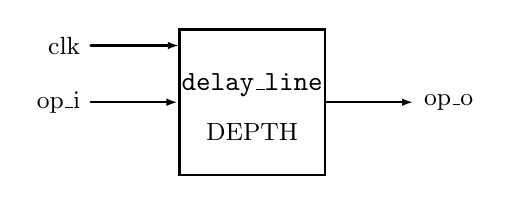
\begin{tikzpicture}[
    font=\small,
    sig/.style={\systolicarrowstyle, line width=0.9pt, line cap=round, line join=round},
    cell/.style={draw, line width=1.0pt, minimum size=1.85cm}
]
  \node[cell] (cellbox) at (0,0) {};
  \node[font=\ttfamily] at ($(cellbox.center)+(0,0.22)$) {delay\_line};
  \node at ($(cellbox.center)+(0,-0.38)$) {$\text{DEPTH}$};

  \draw[sig] (-2.05,0) node[left] {$\text{op\_i}$} -- (cellbox.west);
  \draw[sig] (cellbox.east) -- (2.05,0) node[right] {$\text{op\_o}$};
  \draw[sig] (-2.05,0.72) node[left] {$\text{clk}$} -- (-0.925,0.72);
\end{tikzpicture}%
}

\newcommand{\drawtoprowfeeder}{%
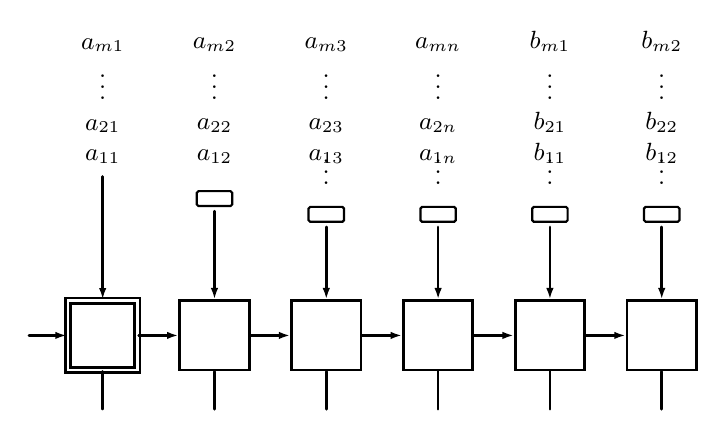
\begin{tikzpicture}[
    font=\small,
    sig/.style={\systolicarrowstyle, line width=0.9pt, line cap=round, line join=round},
    sigline/.style={line width=0.9pt, line cap=round, line join=round},
    meshcol/.style={draw, line width=1.0pt, minimum size=8.8mm, inner sep=0pt},
    meshdiag/.style={draw, double, double distance=0.95pt, line width=0.95pt, minimum size=8.8mm, inner sep=0pt},
    feeddelay/.style={draw, fill=white, line width=0.8pt, minimum width=4.5mm, minimum height=1.9mm, inner sep=0pt},
    feedtxt/.style={align=center, inner sep=0pt}
]
  \def\pitch{1.42}
  \def\stub{0.48}

  \foreach \c in {0,...,5} {
    \pgfmathsetmacro{\x}{\pitch * \c}
    \ifnum\c=0
      \node[meshdiag] (topcell-\c) at (\x,0) {};
    \else
      \node[meshcol] (topcell-\c) at (\x,0) {};
    \fi
  }

  \draw[sig] ([xshift=-\stub cm]topcell-0.west) -- (topcell-0.west);
  \foreach \c/\d in {0/1,1/2,2/3,3/4,4/5} {
    \draw[sig] (topcell-\c.east) -- (topcell-\d.west);
  }
  \foreach \c in {0,...,5} {
    \draw[sigline] (topcell-\c.south) -- ([yshift=-\stub cm]topcell-\c.south);
  }

  \node[feedtxt] (feed-0) at ([yshift=2.55cm]topcell-0.north)
    {$\begin{matrix} a_{m1}\\ \vdots\\ a_{21}\\ a_{11} \end{matrix}$};
  \draw[sig] ([yshift=-0.08cm]feed-0.south) -- (topcell-0.north);

  \node[feedtxt] (feed-1) at ([yshift=2.55cm]topcell-1.north)
    {$\begin{matrix} a_{m2}\\ \vdots\\ a_{22}\\ a_{12} \end{matrix}$};
  \node[feeddelay,rounded corners=0.6pt] (pad-1) at ([yshift=1.28cm]topcell-1.north) {};
  \draw[sig] ([yshift=-0.05cm]pad-1.south) -- (topcell-1.north);

  \node[feedtxt] (feed-2) at ([yshift=2.55cm]topcell-2.north)
    {$\begin{matrix} a_{m3}\\ \vdots\\ a_{23}\\ a_{13} \end{matrix}$};
  \node at ([yshift=1.72cm]topcell-2.north) {$\vdots$};
  \node[feeddelay,rounded corners=0.6pt] (pad-2) at ([yshift=1.08cm]topcell-2.north) {};
  \draw[sig] ([yshift=-0.05cm]pad-2.south) -- (topcell-2.north);

  \node[feedtxt] (feed-3) at ([yshift=2.55cm]topcell-3.north)
    {$\begin{matrix} a_{mn}\\ \vdots\\ a_{2n}\\ a_{1n} \end{matrix}$};
  \node at ([yshift=1.72cm]topcell-3.north) {$\vdots$};
  \node[feeddelay,rounded corners=0.6pt] (pad-3) at ([yshift=1.08cm]topcell-3.north) {};
  \draw[sig] ([yshift=-0.05cm]pad-3.south) -- (topcell-3.north);

  \node[feedtxt] (feed-4) at ([yshift=2.55cm]topcell-4.north)
    {$\begin{matrix} b_{m1}\\ \vdots\\ b_{21}\\ b_{11} \end{matrix}$};
  \node at ([yshift=1.72cm]topcell-4.north) {$\vdots$};
  \node[feeddelay,rounded corners=0.6pt] (pad-4) at ([yshift=1.08cm]topcell-4.north) {};
  \draw[sig] ([yshift=-0.05cm]pad-4.south) -- (topcell-4.north);

  \node[feedtxt] (feed-5) at ([yshift=2.55cm]topcell-5.north)
    {$\begin{matrix} b_{m2}\\ \vdots\\ b_{22}\\ b_{12} \end{matrix}$};
  \node at ([yshift=1.72cm]topcell-5.north) {$\vdots$};
  \node[feeddelay,rounded corners=0.6pt] (pad-5) at ([yshift=1.08cm]topcell-5.north) {};
  \draw[sig] ([yshift=-0.05cm]pad-5.south) -- (topcell-5.north);
\end{tikzpicture}%
}

\newcommand{\drawbottomrowdataout}{%
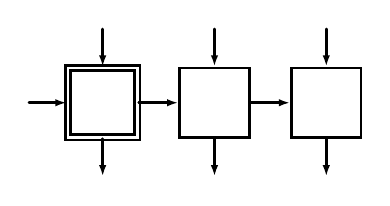
\begin{tikzpicture}[
    font=\small,
    sig/.style={\systolicarrowstyle, line width=0.9pt, line cap=round, line join=round},
    meshcol/.style={draw, line width=1.0pt, minimum size=8.8mm, inner sep=0pt},
    meshdiag/.style={draw, double, double distance=0.95pt, line width=0.95pt, minimum size=8.8mm, inner sep=0pt}
]
  \def\pitch{1.42}
  \def\stub{0.48}

  \node[meshdiag] (botcell-0) at (0,0) {};
  \node[meshcol] (botcell-1) at (\pitch,0) {};
  \node[meshcol] (botcell-2) at ({2*\pitch},0) {};

  \draw[sig] ([xshift=-\stub cm]botcell-0.west) -- (botcell-0.west);
  \draw[sig] (botcell-0.east) -- (botcell-1.west);
  \draw[sig] (botcell-1.east) -- (botcell-2.west);

  \foreach \c in {0,1,2} {
    \draw[sig] ([yshift=\stub cm]botcell-\c.north) -- (botcell-\c.north);
    \draw[sig] (botcell-\c.south) -- ([yshift=-\stub cm]botcell-\c.south);
  }
\end{tikzpicture}%
}

\newcommand{\drawtrapeziodmeshmthreefourtwo}{%
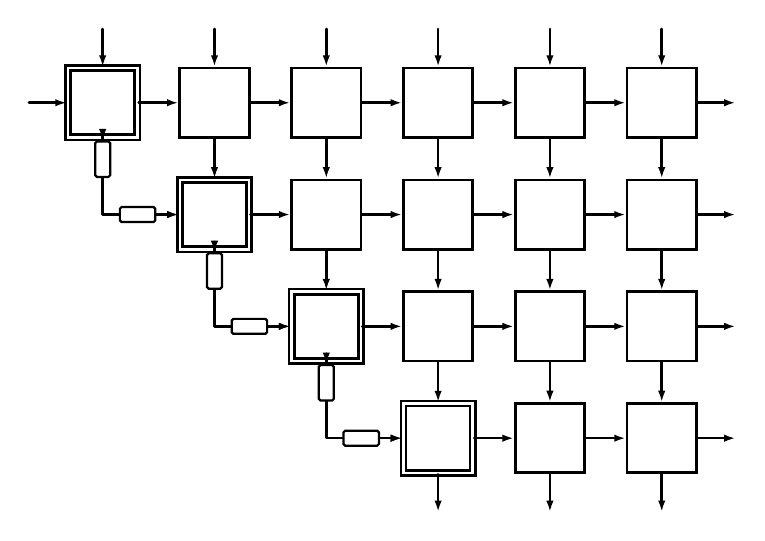
\begin{tikzpicture}[
    font=\small,
    sig/.style={\systolicarrowstyle, line width=0.9pt, line cap=round, line join=round},
    sigline/.style={line width=0.9pt, line cap=round, line join=round},
    meshcol/.style={draw, line width=1.0pt, minimum size=8.8mm, inner sep=0pt},
    meshdiag/.style={draw, double, double distance=0.95pt, line width=0.95pt, minimum size=8.8mm, inner sep=0pt},
    delayh/.style={draw, fill=white, line width=0.8pt, minimum width=1.9mm, minimum height=4.5mm, inner sep=0pt},
    delayv/.style={draw, fill=white, line width=0.8pt, minimum width=4.5mm, minimum height=1.9mm, inner sep=0pt}
]
  \def\pitch{1.42}
  \def\stub{0.48}

  \foreach \r in {0,1,2,3} {
    \foreach \c in {\r,...,5} {
      \pgfmathsetmacro{\x}{\pitch * \c}
      \pgfmathsetmacro{\y}{-\pitch * \r}
      \ifnum\c=\r
        \node[meshdiag] (cell-\r-\c) at (\x,\y) {};
      \else
        \node[meshcol] (cell-\r-\c) at (\x,\y) {};
      \fi
    }
  }

  % top-edge data inputs
  \foreach \c in {0,...,5} {
    \draw[sig] ([yshift=\stub cm]cell-0-\c.north) -- (cell-0-\c.north);
  }

  % vertical data propagation through active columns
  \foreach \c in {1,...,5} {
    \draw[sig] (cell-0-\c.south) -- (cell-1-\c.north);
  }
  \foreach \c in {2,...,5} {
    \draw[sig] (cell-1-\c.south) -- (cell-2-\c.north);
  }
  \foreach \c in {3,...,5} {
    \draw[sig] (cell-2-\c.south) -- (cell-3-\c.north);
  }

  % bottom-edge observations
  \draw[sig] (cell-0-0.south) -- ([yshift=-\stub cm]cell-0-0.south);
  \draw[sig] (cell-1-1.south) -- ([yshift=-\stub cm]cell-1-1.south);
  \draw[sig] (cell-2-2.south) -- ([yshift=-\stub cm]cell-2-2.south);
  \foreach \c in {3,...,5} {
    \draw[sig] (cell-3-\c.south) -- ([yshift=-\stub cm]cell-3-\c.south);
  }

  % left-edge op inputs
  \foreach \r in {0,1,2,3} {
    \draw[sig] ([xshift=-\stub cm]cell-\r-\r.west) -- (cell-\r-\r.west);
  }

  % horizontal op propagation across rows
  \foreach \c/\d in {0/1,1/2,2/3,3/4,4/5} {
    \draw[sig] (cell-0-\c.east) -- (cell-0-\d.west);
  }
  \foreach \c/\d in {1/2,2/3,3/4,4/5} {
    \draw[sig] (cell-1-\c.east) -- (cell-1-\d.west);
  }
  \foreach \c/\d in {2/3,3/4,4/5} {
    \draw[sig] (cell-2-\c.east) -- (cell-2-\d.west);
  }
  \foreach \c/\d in {3/4,4/5} {
    \draw[sig] (cell-3-\c.east) -- (cell-3-\d.west);
  }

  % right-edge op outputs
  \foreach \r in {0,1,2,3} {
    \draw[sig] (cell-\r-5.east) -- ([xshift=\stub cm]cell-\r-5.east);
  }

  % delayed diagonal-to-diagonal path between pe_diag cells
  \foreach \r/\rn in {0/1,1/2,2/3} {
    \coordinate (diag-start-\r) at (cell-\r-\r.south);
    \coordinate (diag-entry-\r) at ([xshift=-0.18cm]cell-\rn-\rn.west);
    \coordinate (diag-turn-\r) at (diag-start-\r |- diag-entry-\r);
    \node[delayh,rounded corners=0.6pt] (diag-dh-\r) at ([yshift=-0.26cm]cell-\r-\r.south) {};
    \node[delayv,rounded corners=0.6pt] (diag-dv-\r) at ([xshift=-0.34cm]diag-entry-\r) {};

    \draw[sig] (diag-start-\r) -- (diag-dh-\r.north);
    \draw[sigline] (diag-dh-\r.south) -- (diag-turn-\r) -- (diag-dv-\r.west);
    \draw[sig] (diag-dv-\r.east) -- (diag-entry-\r) -- (cell-\rn-\rn.west);
  }
\end{tikzpicture}%
}
